\documentclass[border=10pt]{standalone}

\usepackage{tikz}
\usepackage{tikzsymbols}
\usetikzlibrary{calc,patterns,shapes.geometric}

\def\centerarc[#1](#2)(#3:#4:#5){\draw[#1] ($(#2)+({#5*cos(#3)},{#5*sin(#3)})$) arc (#3:#4:#5);}

\begin{document}
	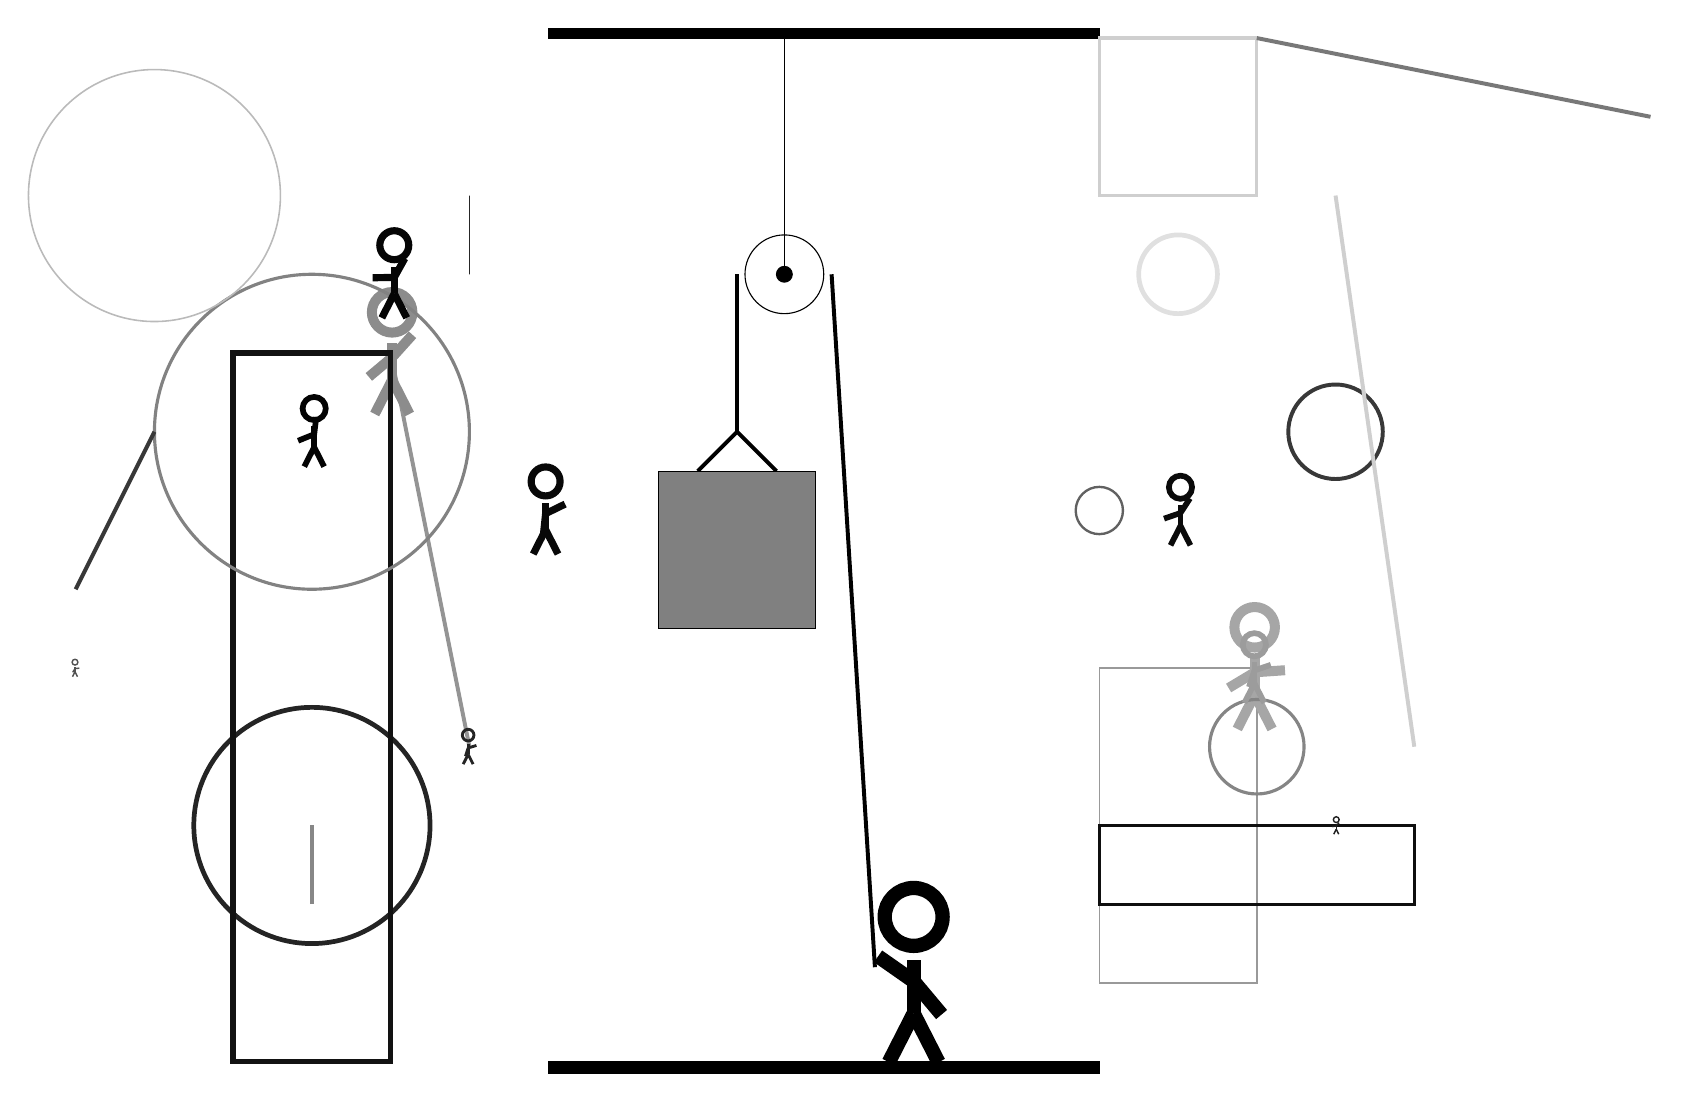
\begin{tikzpicture}
		%%%%% START %%%%%
		
		\draw[fill=black] (-2, 10) rectangle (5, 10.125);
		
		\draw (1, 7) circle (0.5);
		\draw[fill=black] (1, 7) circle (0.1);
		\draw (1, 10) -- (1, 7);
		
		\draw[line width=0.5mm] (-0.1, 4.5) -- (0.4, 5.0) -- (0.9, 4.5);
		\draw[fill=black!50] (-0.6, 4.5) rectangle (1.4, 2.5);
		
		\draw[line width=0.2mm, color=black!40] (5, -2) rectangle (7, 2);
		
		\draw[line width=0.5mm, color=black!42](-4, 6) -- (-3, 1);
		\draw [line width=0.5mm, color=black!78](8, 5) circle (0.6);
		\draw [line width=0.2mm, color=black!42](-6, 10) circle (0.0);
		\draw [line width=0.6mm, color=black!12](6, 7) circle (0.5);
		\node[line width=0.3mm, color=black!35] at (7, 2) {\Strichmaxerl[7][31][4]};
		
		\draw [line width=0.6mm, color=black!86](-5, 0) circle (1.5);
		
		\node[line width=0.5mm, color=black!96] at (6, 4) {\Strichmaxerl[4][19][57]};
		\draw[line width=0.2mm, color=black!85] (-3, 8) rectangle (-3, 7);
		
		\draw[line width=0.4mm, color=black!94] (5, -1) rectangle (9, 0);
		
		\draw[line width=0.4mm, color=black!19] (7, 10) rectangle (5, 8);
		\node[line width=0.3mm, color=black!45] at (-4, 6) {\Strichmaxerl[7][40][48]};
		\draw [line width=0.3mm, color=black!62](5, 4) circle (0.3);
		
		\draw[line width=0.7mm, color=black!93] (-4, 6) rectangle (-6, -3);
		\draw [line width=0.4mm, color=black!48](7, 1) circle (0.6);
		\draw[line width=0.5mm, color=black!19](9, 1) -- (8, 8);
		
		\draw [line width=0.4mm, color=black!49](-5, 5) circle (2.0);
		\node[line width=0.6mm, color=black!68] at (-8, 2) {\Strichmaxerl[1][58][6]};
		\node[line width=0.6mm, color=black!98] at (-4, 7) {\Strichmaxerl[5][1][61]};
		
		\draw[line width=0.5mm, color=black!78](-7, 5) -- (-8, 3);
		\node[line width=0.2mm, color=black!99] at (-5, 5) {\Strichmaxerl[4][22][83]};
		\draw[line width=0.5mm, color=black!53](7, 10) -- (12, 9);
		
		\draw[line width=0.5mm, color=black!47](-5, -1) -- (-5, 0);
		\node[line width=0.7mm, color=black!39] at (7, 2) {\Strichmaxerl[4][72][19]};
		\node[line width=0.3mm, color=black!88] at (8, 0) {\Strichmaxerl[1][6][51]};
		
		\draw [line width=0.2mm, color=black!27](-7, 8) circle (1.6);
		
		\node[line width=0.7mm, color=black!86] at (-3, 1) {\Strichmaxerl[2][72][17]};
		\node[line width=0.4mm, color=black!97] at (-2, 4) {\Strichmaxerl[5][84][26]};
		
		
		\draw[line width=0.5mm] (0.4, 7) -- (0.4, 5.0);
		\centerarc[line width=0.5mm](1, 7)(0:180:0.6);
		\draw[line width=0.5mm](1.6, 7) -- (2.15, -1.8);
		
		\node at (2.6, -1.9) {\Strichmaxerl[10][-35][-50]};
		
		\draw[fill=black] (-2, -3) rectangle (5, -3.15);
		
		%%%%% END %%%%%
	\end{tikzpicture}
\end{document}